% This is the aspauthor.tex LaTeX file
% Copyright 2010, Astronomical Society of the Pacific Conference Series

\documentclass[11pt,twoside]{article}

\usepackage{asp2010}

\resetcounters

\bibliographystyle{asp2010}

\markboth{Rauch et al.}{Spectral Analysis in the Virtual Observatory}

\begin{document}

\title{Spectral Analysis in the Virtual Observatory}
\author{Thomas Rauch, Nicole Reindl, and Ellen M\"uller-Ringat}
\affil{Institute for Astronomy and Astrophysics,
       Kepler Center for Astro and Particle Physics,
       Eberhard Karls University,
       Sand 1, 
       72076 T\"ubingen,
       Germany}

\begin{abstract}
In a collaboration of the \emph{German Astrophysical Virtual Observatory}
and \emph{AstroGrid-D}, the \emph{German Astronomy Community Grid},
we provide the registered \emph{Virtual Observatory} service \emph{TheoSSA} for the access and the 
calculation of stellar spectral-energy distributions.
Recently, we extended this service to consider opacities of H, He, C, N, O, 
Ne, and Mg. We demonstrate the impact of Ne and Mg on model atmospheres. 
\end{abstract}


\section{Spectral Energy Distributions }
\label{sect:seds}

The \emph{German Astrophysical Virtual Observatory} (\emph{GAVO}) is the German contribution to the 
\emph{International Virtual Observatory Alliance} (\emph{IVOA}). The ambitious goal of the \emph{Virtual 
Observatory} (\emph{VO}) initiative is to help astronomers to easily access data stored in various 
data centers which are distributed around the world. Furthermore it strives to 
standardize the handling and retrieval of archived data. Also the development of web 
interfaces and standalone tools for accessing, querying, and visualizing the
data is an important task, that \emph{GAVO} pursues.

The \emph{T\"ubingen NLTE Model-Atmosphere Package} 
\citep[\emph{TMAP},][]{werneretal2003, rauchdeetjen2003} is a 
sophisticated model-atmosphere code 
\citep[e.g\@.][]{rauchetal2007},
that was developed over the last 26 years 
and uses the most recent atomic data from the model-atom database
\emph{TMAD}\footnote[1]{\url{http://astro.uni-tuebingen.de/~TMAD}}.
Elements from hydrogen to xenon can be included into the calculations 
\citep{rauch2003,werneretal2012,rauchetal2012}. 
Within the \emph{GAVO} project, \emph{TMAP} was made accessible \citep{rauchringat2011}.
Already calculated spectral energy distributions
(SEDs) can be downloaded via \emph{TheoSSA} and enable a fast and 
easy spectral analysis. It is controlled via a web interface where the fundamental 
parameters can be entered. The user receives a list of SEDs within the requested 
parameter range. For a more detailed analysis, the \emph{VO} service \emph{TMAW} (Fig.~\ref{fig:tmaw}), the 
web interface of \emph{TMAP}, can be employed to calculate individual atmosphere models. 
Effective temperatures between 20\,kK and about 300\,kK and surface gravities
$4 \leq \log (g / \mathrm{cm/s^2}) \leq 9$ can be chosen.
In the beginning,  \emph{TMAW} considered opacities of the elements H+He+C+N+O only.
We have now extended \emph{TMAW} to include Ne+Mg.
Depending on the number of models in the \emph{TMAW} queue, the requested SEDs 
will be calculated within a few days. It is even possible to calculate
extended grids of SEDs on compute resources of AstroGrid-D\footnote[2]{\url{http://www.gac-grid.net/}}.


\begin{landscape}
\begin{figure}[ht!]\centering
\includegraphics[width=18.5cm]{p24_f1.eps}
\caption{Web interface of \emph{TMAW}.}
\label{fig:tmaw}
\end{figure}
\end{landscape}


\begin{figure}[ht!]\centering
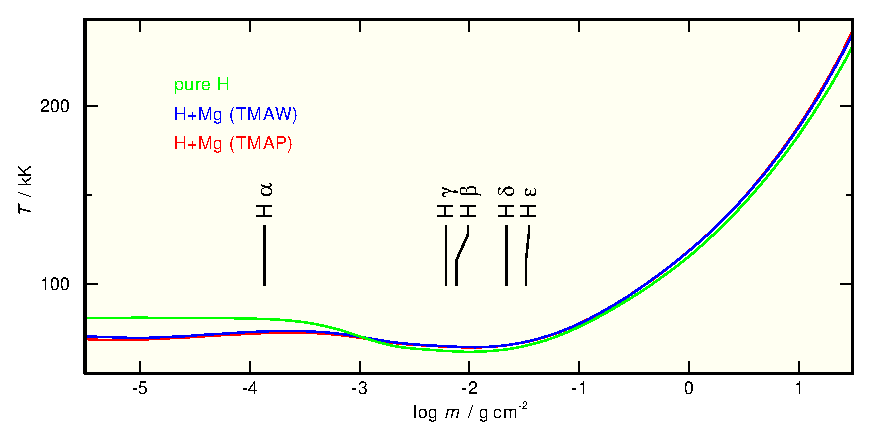
\includegraphics[width=0.8\textwidth]{p24_f2.eps}
\caption{The impact of Mg on the temperature structure of the model atmosphere
         \citep[$T_\mathrm{eff}=60\,\mathrm{kK}$, $\log g = 7$, solar abundances,][]{asplundetal2009}.
         The formation depths of the line cores of H\,{\sc i} lines are indicated.}
\label{fig:Tstruc}
\end{figure}


\section{The impact of neon and magnesium on stellar model atmospheres}
\label{sect:nemg}

The \emph{TMAW} service had hitherto been restricted
to H+Ne+C+N+O models in order to deliver SEDs within one day.
We recently included the next abundant elements, namely Mg and Ne,
in the calculations. A ``full'' model needs now about two or three days,
depending on the machine where its calculation is performed.

To study the impact of Mg and Ne in detail, we calculated pure hydrogen models 
and for comparison models that include either Mg or Ne in addition, using 
\emph{TMAW} and \emph{TMAP}. In the \emph{TMAP} model, more detailed model atoms 
were considered (181 levels treated in NLTE with 479 line transitions)
and they were calculated until the absolute relative corrections are smaller 
than $10^{-4}$. To ensure reasonable calculation times,  the \emph{TMAW} model 
considered only 89 levels in NLTE and 132 lines \citep[cf\@.][]{rauchringat2012}.

Ne and Mg have a significant impact on the temperature structure of the entire atmosphere.
Figure~\ref{fig:Tstruc} shows that Mg causes a strong decrease of the temperature in the outer
atmosphere for $\log m \leq -3$. Since e.g\@. the H\,$\alpha$ line core is formed at 
$\log m \approx -3.9$, the impact on this line is particularly strong.

We examined the optical hydrogen lines that are often used to determine the effective 
temperature and / or the surface gravity of a star. In Fig.~\ref{fig:HMg}, a pure 
hydrogen model is compared with a \emph{TMAW} and a \emph{TMAP} model that also include 
Mg \citep[$T_\mathrm{eff}=60\,\mathrm{kK}$, $\log g = 7$, solar abundances,][]{asplundetal2009}.
The difference between the pure hydrogen model and the 
\emph{TMAP} model is always larger than the difference between the \emph{TMAW} and 
the \emph{TMAP} model. The strength of the central emission of the H\,$\alpha$ line differs 
only by $\Delta \approx 0.01$ (in relative flux) between the \emph{TMAW} and \emph{TMAP} models, 
whereas the pure hydrogen model and the \emph{TMAW} differ by $\Delta \approx 0.10$.


\begin{figure}[ht!]\centering
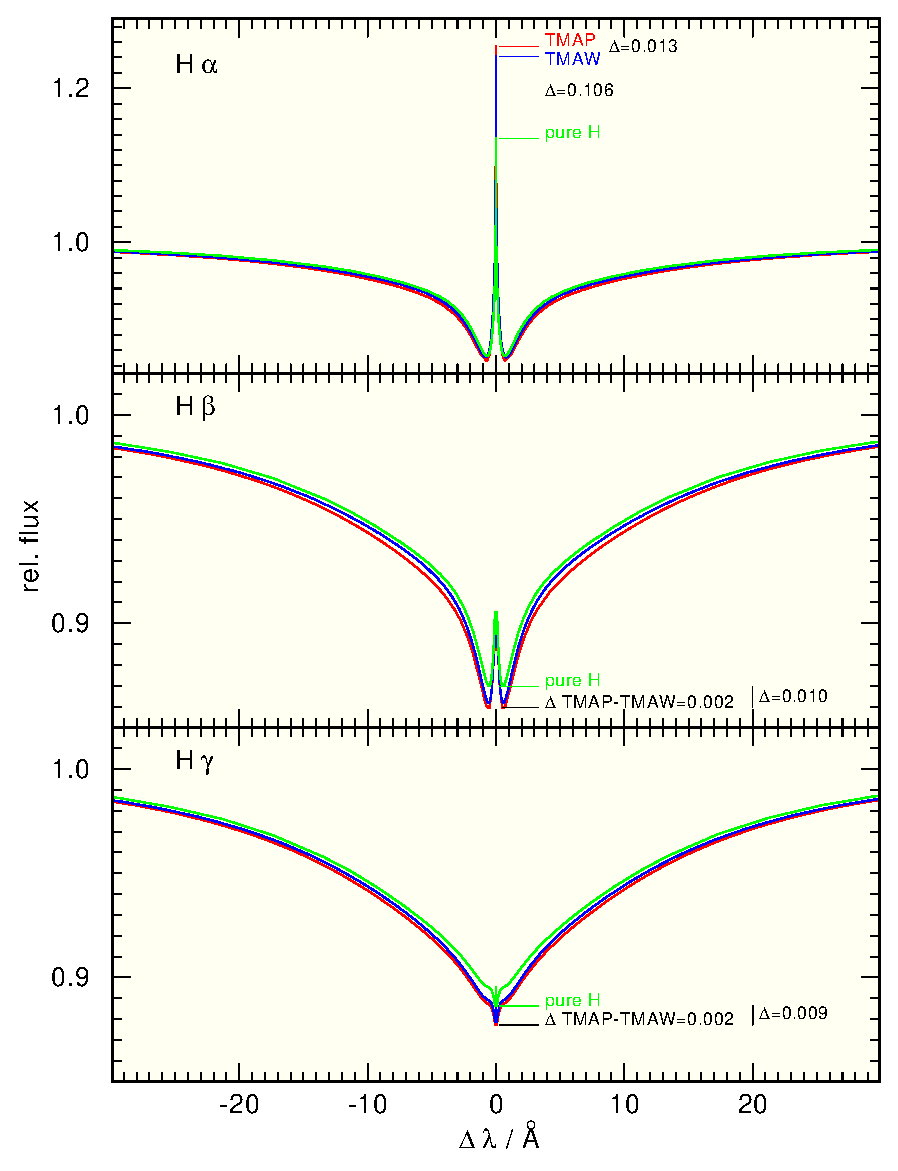
\includegraphics[width=0.65\textwidth]{p24_f3.eps}
\caption{The impact of Mg on optical H\,{\sc i} line profiles.}
\label{fig:HMg}
\end{figure}


\acknowledgements 
TR is supported by the German Aerospace Center (DLR, grant 05\,OR\,0806), 
NR and EMR by the German Research Foundation (DFG, grant WE 1312/41-1).
We thank the \emph{GAVO} and \emph{AstroGrid-D} teams for support.


\bibliography{../../editor}


\end{document}
